\documentclass[11pt
  , a4paper
  , article
  , oneside
  %  , twoside
  , showtrims
 % , draft
]{memoir}

\usepackage{essdocs}
\usepackage[numbers]{natbib}
\usepackage[autostyle]{csquotes}

\setsecnumdepth{subsection}

\begin{document}
%\frontmatter
%% ESS Document Description
%%
\essdocdesc{Engineering Manual}

%% ESS Document Number
%%
\essdocnum{ESS-0508480}

%% Date
%%
\date{\today}

%% ESS Document Revision Number
%%
\essdocrev{0.3}

%% ESS Document State
%%
\essdocstate{Early Draft}

%% ESS Document Classification
%%
\essdocclass{ESS Use Only}

%% Document Title
%%
\title{ICS Engineering Manual}
\subtitle{for MRF MTCA-EVR-300(U)}
%% Document Author(s), if more than one author,
%% use \newline instead of \\ or \linebreak in order to seperate them
\author{Javier Cereijo Garcia \newline Jeong Han Lee }

%% Document Reviewer(s) if more than one reviewer,
%% use \newline instead of \\ or \linebreak in order to seperate them
%\reviewer{Timo Korhonen (Chief Engineer) \newline Timo Korhonen (Chief Engineer)}
\reviewer{TBD}
%% Document Owner(s) if more than one owner,
%% use \newline instead of \\ or \linebreak in order to seperate them
\owner{ICS}

%% Document Approver(s) if more than one approver,
%% use \newline instead of \\ or \linebreak in order to seperate them
\approver{ICS}

\showtrimson

\esstitle
\newpage
\tableofcontents
\newpage

%\mainmatter


%%% Actual Document Start at below
\chapter{Overview}
At European Spallation Source (ESS), Integrated Control System (ICS) uses the Micro Research Finland (MRF) Timing System{\footnote{\url{http://www.mrf.fi/}}} as its timing system of the ESS site. The consistent and up-to-date engineering manual is essential for the ESS Timing system.


\section{Scope}
\begin{itemize}
\item This document identifies one of the MRF Timing Event Receivers (EVR) that needs to be configured for an ESS subsystem that needs synchronous frequencies, trigger signals and sequences of events \cite{MRFEVENTSYSTEMDC}.
\item This document provides the generic description of the MRF MTCA-EVR-300(U) and its interface board (IFB-300). In addition, it affords the minimal, essential, and generic information for the system configuration.
\item The purpose of this document is to describe the engineering procedure and troubleshooting about how the MRF MTCA-EVR-300(U) board will be integrated in cooperation with the new ESS EPICS Environment (E3).
\item This document attempts to maintain consistency with existing ESS Timing system hardware as far as possible.
\end{itemize}
\textbf{Note that this is a very early draft document and should be updated as development progresses.}


\section{Target Audience}
This document is targeted to ICS engineers and technical stakeholders of the ESS timing system. It is assumed that the target audience has a technical background in the MRF Timing System, the EPICS development, and a Linux environment.



\chapter{System Description}
MRF Technical Reference \citep[see][p45]{MRFEVENTSYSTEMDC} explained Event Receivers and wrote :
\blockquote{\textit{Event Receivers decode timing events and signals from an optical event stream transmitted by an Event Generator. Events and signals are received at predefined rate the event clock that is usually divided down from an accelerators main RF reference. The event receivers lock to the phase event clock of the Event Generator and are thus phase locked to the RF reference. Event Receivers convert event codes transmitted by an Event Generator to hardware outputs. They can also generate software interrupts and store the event codes with globally distributed timestamps into FIFO memory to be read by a CPU.}}

ICS uses and will use the following different types of EVR :
\begin{itemize}
\item MTCA-EVR-300(U)
\item PCIe-EVR-300DC
\end{itemize}

The scope of this document is to cover the MTCA-EVR-300(U) board.


\section{MTCA-EVR-300(U)}
Figure~\ref{fig:mtca-evr300} shows the rough physical dimensions $181\times 148~\mathrm{mm}{}^2$ of the MTCA-EVR-300 card.

\begin{figure}[!htb]
  \centering
  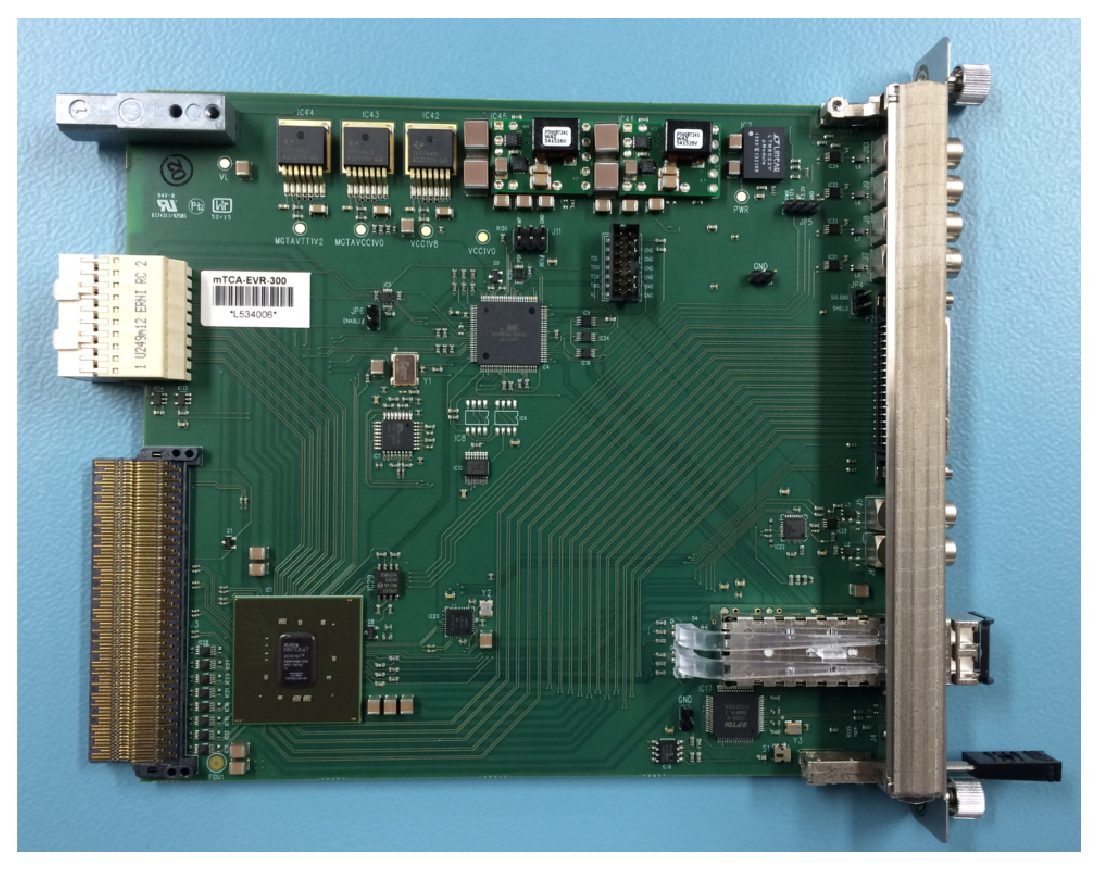
\includegraphics[width=0.99\textwidth]{./pictures/mtca_evr_300.eps}
  \caption{
    MRF MTCA-EVR-300 board.
  }
  \label{fig:mtca-evr300}
\end{figure}


The MTCA-EVR-300  has a SFP transceiver as an input from EVG and several outputs: 4 front panel outputs, 16 front universal outputs (through the IFB-300 extension board) and 40 rear outputs. The initial 32 rear outputs map to the RTM connector, the last 8 rear outputs map to the MTCA backplane. The 16 front universal outputs are implemented through a micro-SCSI type connector for an interface board IFB-300. The IFB-300 has eight Universal I/O slots, each of them accommodating 2 outputs/inputs, shown in Figure~\ref{fig:ifb-300}. With different type of MRF Universal I/O modules, each slot can be used as an unique trigger or event signal source.

\begin{figure}[!htb]
  \centering
  \includegraphics{./pictures/ifb-300.eps}
  \caption{
    MRF Interface Board IFB 300 Front Panel \cite{MRFEVENTSYSTEMDC}.
  }
  \label{fig:ifb-300}
\end{figure}

The MTCA-EVR-300U is identical to the MTCA-EVR-300 except for the fact that it replaces the micro-SCSI connector for 2 Universal I/O slots.



\clearpage
\chapter{System Environment}
Before describing the engineering procedure for an E3 integration of the MRF MTCA-EVR-300(U) board, it is mandatory to have proper system environment that consists of specific hardware and software lists. Here we will show the hardware and software lists, their block diagrams, and their setup in the ICS lab at ESS. The information shown in this chapter is used in the ICS Lab at ESS.


\section{Hardware}
Table~\ref{table:hwlist} shows the hardware list. The form factor and version of EVG can be changeable. It is assumed that the proper working EVG system is ready.
\begin{table}[!hb]
  \centering
  \begin{tabular}{l|l}
    \toprule
    Hardware                          & Info               \\\midrule
    MRF MTCA-EVR-300U                 & \texttt{ZZB614}    \\\midrule
    NAT-MCH-PHYS                      & \texttt{AAA573}    \\\midrule
    Concurrent Technologies AMC CPU   & \texttt{ZZB276}    \\\midrule
    Schroff MTCA crate 3U             & \texttt{AAA596}    \\\midrule
    NAT MTCA Power Module 600W        & \texttt{AAA590}    \\\midrule
    MRF cPCI-EVG-230                  & \texttt{ZZB790}    \\\midrule
    Ethernet, LEMO and optical cables & LC, Optical 850 nm \\\midrule
    Oscilloscope                      & \texttt{ZZB406}    \\\bottomrule
  \end{tabular}
  \caption[]{Hardware List.}
  \label{table:hwlist}
\end{table}

% Figure~\ref{fig:diagram} shows the physical hardware setup and
Figure~\ref{fig:mtca-hw-setup} shows the MTCA-EVR-300 setup in the lab. From left to right, the power supply (different model than shown in Table~\ref{table:hwlist}), MCH, CPU, MTCA-EVR-300 and Struck SIS8300 (not used in this document).
\begin{figure}[!b]
  \centering
  \includegraphics[width=0.8\textwidth]{./pictures/mtca-hw-setup.eps}
  \caption{Hardware Setup in the ICS lab.}
  \label{fig:mtca-hw-setup}
\end{figure}


\clearpage
\section{Software}
Table~\ref{table:swlist} shows the Software list and its environment. It is mandatory to check the kernel version, and the mrf kernel module version. Since the mrfioc2 is dependent upon devlib2 E3 internally, an end-user is unnecessary to check its version explicitly.
\begin{table}[!htb]
  \centering
  \begin{tabular}{l|l}
    \toprule
    Item               & Version Info.                                                      \\\midrule
    CentOS Linux       & \texttt{7.6.1810}                                                  \\\midrule
    Kernel             & \texttt{3.10.0-957.1.3.el7.x86\_64}                                \\\midrule
    mrf kernel module  & version : \texttt{1} / srcversion \texttt{E3290AD048B5B57D2EAA55E} \\\midrule
    E3 require         & \texttt{3.0.4}                                                     \\\midrule
    EPICS Base         & \texttt{3.15.5}                                                    \\\midrule
    mrfioc2            & E3 module ver. \texttt{2.2.0-rc4}                                  \\\midrule
    devlib2            & E3 module ver. \texttt{2.9.0}                                      \\\bottomrule
  \end{tabular}
  \caption[]{Software and its version information.}
  \label{table:swlist}
\end{table}


\section{EVR Firmware}
Table~\ref{table:fwinfo} shows EVR FPGA Firmware Version Register.

\begin{table}[!htb]
  \centering
  \begin{tabular}{p{0.3\linewidth}|c|l}
    \toprule
    EVR FPGA Firmware Version Register              & \multicolumn{2}{c}{\texttt{0x18070207}}             \\\midrule
    Board Type        & EVR                         &  \texttt{0x}\underline{\textbf{1}}\texttt{8070207}  \\\midrule
    Form Factor       & mTCA.4                      &  \texttt{0x1}\underline{\textbf{8}}\texttt{070207}  \\\midrule
    EVR Subrelease ID & 7                           &  \texttt{0x18}\underline{\textbf{07}}\texttt{0207}  \\\midrule
    EVR Firmware ID   & Delay Compensation Firmware &  \texttt{0x1807}\underline{\textbf{02}}\texttt{07}  \\\midrule
    EVR Revision ID   & 7                           &  \texttt{0x180702}\underline{\textbf{07}}           \\\bottomrule
  \end{tabular}
  \caption[]{EVR FPGA Firmware Version Register in Reference \citep[see][p66]{MRFEVENTSYSTEMDC}.}
  \label{table:fwinfo}
\end{table}



\clearpage
\chapter{Engineering Procedure}
This chapter provides the minimal information to configure the EVR board properly.


\section{System Installation}
Figure~\ref{fig:mtca-hw-setup} shows the glimpse of what system might be like in a Lab. \textbf{Note that the cable between the mTCA-EVR-300 and IFB-300 (not shown in the figure) should be connected, disconnected, or both only when powered down}. Please see the detail information in Reference \citep[][p54]{MRFEVENTSYSTEMDC}.

It is assumed that the MTCA-EVR-300(U) is installed in a crate with a CPU running CentOS 7 with E3. For more information on E3, please check {\footnote{\url{https://github.com/icshwi/e3training}}.


\section{mTCA-EVR-300(U) Board Identification}

\subsection{Fixing PCI IDs}
The PCI ID list does not include the MRF products. It can be updated as follows:
\begin{itemize}
\item Cloning the sort of ESS customized PCI.IDS db:
\begin{lstlisting}[style=termstyle]
timinguser@icslab-ts03: ics_gitsrc$ git clone https://github.com/jeonghanlee/pciids
\end{lstlisting}
\item Replace the pci.ids file:
\begin{lstlisting}[style=termstyle]
timinguser@icslab-ts03: pciids (master)$ bash replace-pciids.bash
centos was determined.
[sudo] password for timinguser:
\end{lstlisting}
\item Check MRF products by the vendor's id (1a3e):
\begin{lstlisting}[style=termstyle]
timinguser@icslab-ts03: pciids (master)$ lspci -nmmn | grep -E "\<(1a3e)"
"0b:00.0 "Signal processing controller [1180]" "Xilinx Corporation [10ee]" "XILINX PCI DEVICE [7011]" "Micro-Research Finland Oy [1a3e]" "MTCA Event Receiver 300 [132c]"
\end{lstlisting}
\end{itemize}

\subsection{Kernel module}
The MTCA-EVR-300(U) needs a kernel module to work. It can be installed by simply running some commands. Do the following:
\begin{itemize}
\item Go to your e3-mrfioc2 sources directory:
\begin{lstlisting}[style=termstyle]
timinguser@icslab-ts03: ~$ cd e3/e3-mrfioc2
\end{lstlisting}
\item Install the kernel module:
\begin{lstlisting}[style=termstyle]
timinguser@icslab-ts03: e3-mrfioc2 (master)$ make dkms_add
/epics/base-3.15.5/bin/linux-x86_64/msi -M name="mrfioc2" -M  version="2.2.0-rc4" -M kmod_name="mrf" /home/timinguser/e3/e3-mrfioc2/dkms/dkms_with_msi.conf.in > /home/timinguser/e3/e3-mrfioc2/dkms/dkms_with_msi.conf
sudo install -d /usr/src/mrfioc2-2.2.0-rc4
sudo cp -r /home/timinguser/e3/e3-mrfioc2/mrfioc2/mrmShared/linux/* /usr/src/mrfioc2-2.2.0-rc4/
sudo /usr/sbin/dkms add -m mrfioc2 -v 2.2.0-rc4

Creating symlink /var/lib/dkms/mrfioc2/2.2.0-rc4/source ->
                 /usr/src/mrfioc2-2.2.0-rc4

DKMS: add completed.
timinguser@icslab-ts03: e3-mrfioc2 (master)$ make dkms_build
sudo /usr/sbin/dkms build -m mrfioc2 -v 2.2.0-rc4

Kernel preparation unnecessary for this kernel.  Skipping...

Building module:
cleaning build area...
make -j4 KERNELRELEASE=3.10.0-957.1.3.el7.x86_64 -C /lib/modules/3.10.0-957.1.3.el7.x86_64/build M=/var/lib/dkms/mrfioc2/2.2.0-rc4/build modules...
cleaning build area...

DKMS: build completed.
timinguser@icslab-ts03: e3-mrfioc2 (master)$ make dkms_install
sudo /usr/sbin/dkms install -m mrfioc2 -v 2.2.0-rc4

mrf.ko.xz:
Running module version sanity check.
 - Original module
   - No original module exists within this kernel
 - Installation
   - Installing to /lib/modules/3.10.0-957.1.3.el7.x86_64/extra/
Adding any weak-modules

depmod...

DKMS: install completed.
timinguser@icslab-ts03: e3-mrfioc2 (master)$ make setup
KERNEL=="uio*", ATTR{name}=="mrf-pci", MODE="0666"
mrf
rmmod mrf
rmmod parport
rmmod uio
insmod /lib/modules/3.10.0-957.1.3.el7.x86_64/kernel/drivers/parport/parport.ko.xz
insmod /lib/modules/3.10.0-957.1.3.el7.x86_64/kernel/drivers/uio/uio.ko.xz
insmod /lib/modules/3.10.0-957.1.3.el7.x86_64/extra/mrf.ko.xz


It is OK to see "E3/RULES_DKMS:37: recipe for target 'setup' failed"
---------------------------------------------------------------------
crw-rw-rw-. 1 root root 241, 0 Dec 13 10:11 /dev/uio0
crw-rw-rw-. 1 root root 241, 1 Dec 13 10:11 /dev/uio1
---------------------------------------------------------------------
\end{lstlisting}
\item Check kernel module information:
\begin{lstlisting}[style=termstyle]
timinguser@icslab-ts03: pciids (master)$ lsmod |grep mrf
mrf                    18137  0
uio                    19338  1 mrf
parport                46395  1 mrf
timinguser@icslab-ts03: pciids (master)$ modinfo mrf
filename:       /lib/modules/3.10.0-957.1.3.el7.x86_64/extra/mrf.ko.xz
author:         Michael Davidsaver <mdavidsaver@gmail.com>
version:        1
license:        GPL v2
retpoline:      Y
rhelversion:    7.6
srcversion:     E3290AD048B5B57D2EAA55E
alias:          pci:v000010EEd00007011sv00001A3Esd0000232Cbc*sc*i*
alias:          pci:v000010EEd00007011sv00001A3Esd0000132Cbc*sc*i*
alias:          pci:v00001A3Ed0000152Csv00001A3Esd0000152Cbc*sc*i*
alias:          pci:v00001A3Ed0000252Csv00001A3Esd0000252Cbc*sc*i*
alias:          pci:v000010EEd00007011sv00001A3Esd0000172Cbc*sc*i*
alias:          pci:v00001204d0000EC30sv00001A3Esd0000172Cbc*sc*i*
alias:          pci:v000010B5d00009056sv00001A3Esd0000192Cbc*sc*i*
alias:          pci:v000010B5d00009030sv00001A3Esd000011E6bc*sc*i*
alias:          pci:v000010B5d00009030sv00001A3Esd000020E6bc*sc*i*
alias:          pci:v000010B5d00009030sv00001A3Esd000020DCbc*sc*i*
alias:          pci:v000010B5d00009030sv00001A3Esd000010E6bc*sc*i*
depends:        parport,uio
vermagic:       3.10.0-957.1.3.el7.x86_64 SMP mod_unload modversions
parm:           cable:Name of JTAG parallel port cable to emulate (charp)
parm:           interfaceversion:User space interface version (int)
parm:           use_msi:Use MSI if present (default 1, yes) (uint)
\end{lstlisting}
%Check that the source version is the same as shown; it should be if these steps are followed as shown. Otherwise please inform ICS.
\end{itemize}

\subsection{PCI Addressing}
Each PCI device is identified by a domain, a bus, a device, and a function number in Linux. Therefore, in order to initialize the MRF MTCA-EVR-300(U) board in E3, one needs the following information: a bus number, a device number, and a function number. These numbers are the parameters of a \texttt{mrmEvrSetupPCI} function.

One can use \texttt{lspci} to find them as follows:
\begin{lstlisting}[style=termstyle]
timinguser@icslab-ts03: ~$ lspci
...
0b:00.0 Signal processing controller: Xilinx Corporation XILINX PCI DEVICE
...
timinguser@icslab-ts03: ~$ lspci -s 0b:00.0 -vv
0b:00.0 Signal processing controller: Xilinx Corporation XILINX PCI DEVICE
	Subsystem: Micro-Research Finland Oy MTCA Event Receiver 300
	Physical Slot: 6
	Control: I/O+ Mem+ BusMaster+ SpecCycle- MemWINV- VGASnoop- ParErr- Stepping- SERR- FastB2B- DisINTx+
	Status: Cap+ 66MHz- UDF- FastB2B- ParErr- DEVSEL=fast >TAbort- <TAbort- <MAbort- >SERR- <PERR- INTx-
	Latency: 0, Cache Line Size: 64 bytes
	Interrupt: pin A routed to IRQ 70
	Region 0: Memory at c0600000 (32-bit, non-prefetchable) [size=256K]
	Capabilities: <access denied>
	Kernel driver in use: mrf-pci
	Kernel modules: mrf

\end{lstlisting}

And one should identify four number as follows:
\begin{lstlisting}[style=termstyle]
timinguser@icslab-ts03: ~$ lspci -s 0b:00.0 -t
-+-[0000:0b]---00.0
 \-[0000:00]-
\end{lstlisting}
, where \texttt{-+-[0000:0b]---00.0} can be translated to \texttt{-+-}[domain:bus]\texttt{---}device.function. Thus in the above case, three numbers are shown in Table~\ref{table:pciidnumber}.\begin{table}[!htb]
  \centering
  \begin{tabular}{l|l}
    \toprule
    bus      & 0x0b \\\midrule
    device   & 0x00 \\\midrule
    function & 0x00 \\\bottomrule
  \end{tabular}
  \caption[]{MRF MTCA-EVR-300(U) Identification Numbers}
  \label{table:pciidnumber}
\end{table}


\clearpage
\section{EPICS IOC Setup under E3}
In order to start the EPICS IOC for the MRF MTCA-EVR-300(U) under E3, one should consider the following things: 1) the EPICS database file, and 2) the EPICS start-up script. The working directory, where an user can create, e.g., in the ICS Lab,
\begin{lstlisting}[style=termstyle, label={list:pwd}, caption={Working Directory in the ICS lab.} ]
/home/timinguser/e3/e3-mrfioc2/cmds
\end{lstlisting}

\subsection{EPICS Database File}
The database file in E3 is located in the following location:
\begin{lstlisting}[style=termstyle]
/epics/base-3.15.5/require/3.0.4/siteMods/mrfioc2/2.2.0-rc4/db/evr-mtca-300-ess.db
/epics/base-3.15.5/require/3.0.4/siteMods/mrfioc2/2.2.0-rc4/db/evr-mtca-300u-ess.db
\end{lstlisting}

\subsection{Start-Up Script}
Listing~\ref{list:emmtcaevr300.cmd} shows the IOC start-up script which has the MRF MTCA-EVR-300(U) Identification Numbers, as explained in the previous step.

\begin{lstlisting}[
    style=termstyle,
    label={list:emmtcaevr300.cmd},
    caption={Start-up script \texttt{emmtcaevr300.cmd}. Line \ref{pciid0} should be matched to Table~\ref{table:pciidnumber} as \texttt{mrmEvrSetupPCI(\$(DEV1), "bus:device.function")}.}
  ]
require mrfioc2,2.2.0-rc4

epicsEnvSet("IOC", "EMMTCAEVR300")
epicsEnvSet("DEV1", "EVR0")

epicsEnvSet("ESSEvtClockRate"  "88.0525")

mrmEvrSetupPCI("$(DEV1)",  "0b:00.0") (*@\label{pciid0}@*)
dbLoadRecords("evr-mtca-300u-ess.db","EVR=$(DEV1), SYS=$(IOC), D=$(DEV1), FEVT=$(ESSEvtClockRate)")

# needed with software timestamp source w/o RT thread scheduling
var evrMrmTimeNSOverflowThreshold 100000


iocInit()

# Set delay compensation to 70 ns, needed to avoid timestamp issue
dbpf $(IOC)-$(DEV1):DC-Tgt-SP 70
\end{lstlisting}

\subsection{EPICS IOC}
All the EPICS parameters should be run from an E3 session. To start E3, type:
\begin{lstlisting}[style=termstyle]
timinguser@icslab-ts03: cmds (master)$ source /epics/base-3.15.5/require/3.0.4/bin/setE3Env.bash
\end{lstlisting}
All the IOCs and related EPICS commands (caget, caput, camonitor, etc.) should be run from an E3 session.

Under E3, the EPICS IOC can be started via the command \texttt{iocsh.bash emmtcaevr300.cmd}. The output should look like as follows:
\begin{lstlisting}[style=termstyle]
timinguser@icslab-ts03: cmds (master)$ iocsh.bash emmtcaevr300.cmd
#
# Start at "2018-W50-Dec13-1424-03-CET"
#
# Version information:
# European Spallation Source ERIC : iocsh.bash (v0.3.5-58bef31.PID-1619)
#
# --->--> snip -->-->
# Please Use Version and other environment variables
# in order to report or debug this shell
#
# HOSTDISPLAY=""
# WINDOWID=""
# PWD="/home/timinguser/e3/e3-mrfioc2/cmds"
# USER="timinguser"
# LOGNAME="timinguser"
# EPICS_HOST_ARCH="linux-x86_64"
# EPICS_BASE="/epics/base-3.15.5"
# E3_REQUIRE_NAME="require"
# E3_REQUIRE_VERSION="3.0.4"
# E3_REQUIRE_LOCATION="/epics/base-3.15.5/require/3.0.4"
# E3_REQUIRE_BIN="/epics/base-3.15.5/require/3.0.4/bin"
# E3_REQUIRE_DB="/epics/base-3.15.5/require/3.0.4/db"
# E3_REQUIRE_DBD="/epics/base-3.15.5/require/3.0.4/dbd"
# E3_REQUIRE_INC="/epics/base-3.15.5/require/3.0.4/include"
# E3_REQUIRE_LIB="/epics/base-3.15.5/require/3.0.4/lib"
# E3_SITEAPPS_PATH="/epics/base-3.15.5/require/3.0.4/siteApps"
# E3_SITELIBS_PATH="/epics/base-3.15.5/require/3.0.4/siteLibs"
# E3_SITEMODS_PATH="/epics/base-3.15.5/require/3.0.4/siteMods"
# EPICS_DRIVER_PATH="/epics/base-3.15.5/require/3.0.4/siteMods:/epics/base-3.15.5/require/3.0.4/siteApps"
# EPICS_CA_AUTO_ADDR_LIST=""
# EPICS_CA_ADDR_LIST=""
# PATH="/epics/base-3.15.5/require/3.0.4/bin:/epics/base-3.15.5/bin/linux-x86_64:/usr/local/bin:/usr/bin:/usr/local/sbin:/usr/sbin:/home/timinguser/.local/bin:/home/timinguser/bin"
# LD_LIBRARY_PATH="/epics/base-3.15.5/lib/linux-x86_64:/epics/base-3.15.5/require/3.0.4/lib/linux-x86_64:/epics/base-3.15.5/require/3.0.4/siteLibs/linux-x86_64"
# --->--> snip -->-->
#
# Set REQUIRE_IOC for its internal PVs
epicsEnvSet REQUIRE_IOC "REQMOD-58BEF31:ICSLAB--1638"
#
# Set E3_IOCSH_TOP for the absolute path where iocsh.bash is executed.
epicsEnvSet E3_IOCSH_TOP "/home/timinguser/e3/e3-mrfioc2/cmds"
#
#
# Load require module, which has the version 3.0.4
#
dlload /epics/base-3.15.5/require/3.0.4/lib/linux-x86_64/librequire.so
dbLoadDatabase /epics/base-3.15.5/require/3.0.4/dbd/require.dbd
require_registerRecordDeviceDriver
Loading module info records for require
#
# Set E3_CMD_TOP for the absolute path where emmtcaevr300.cmd exists
epicsEnvSet E3_CMD_TOP "/home/timinguser/e3/e3-mrfioc2/cmds"
#
iocshLoad 'emmtcaevr300.cmd',''
require mrfioc2,2.2.0-rc4
Module mrfioc2 version 2.2.0-rc4 found in /epics/base-3.15.5/require/3.0.4/siteMods/mrfioc2/2.2.0-rc4/
Module mrfioc2 depends on devlib2 2.9.0
Module devlib2 version 2.9.0 found in /epics/base-3.15.5/require/3.0.4/siteMods/devlib2/2.9.0/
Loading library /epics/base-3.15.5/require/3.0.4/siteMods/devlib2/2.9.0/lib/linux-x86_64/libdevlib2.so
Loaded devlib2 version 2.9.0
Loading dbd file /epics/base-3.15.5/require/3.0.4/siteMods/devlib2/2.9.0/dbd/devlib2.dbd
Calling function devlib2_registerRecordDeviceDriver
Loading module info records for devlib2
Loading library /epics/base-3.15.5/require/3.0.4/siteMods/mrfioc2/2.2.0-rc4/lib/linux-x86_64/libmrfioc2.so
Loaded mrfioc2 version 2.2.0-rc4
Loading dbd file /epics/base-3.15.5/require/3.0.4/siteMods/mrfioc2/2.2.0-rc4/dbd/mrfioc2.dbd
Calling function mrfioc2_registerRecordDeviceDriver
Loading module info records for mrfioc2
epicsEnvSet("IOC", "EMMTCAEVR300")
epicsEnvSet("DEV1", "EVR0")
#epicsEnvSet("MainEvtCODE" "14")
#epicsEnvSet("HeartBeatEvtCODE"   "122")
epicsEnvSet("ESSEvtClockRate"  "88.0525")
mrmEvrSetupPCI("EVR0",  "0b:00.0")
Notice: devPCIFindSpec() expect B:D.F in hex
Device EVR0  b:0.0 slot=6
Using IRQ 70
FWVersion 0x18070207
Found version 519
Found SFP EEPROM
Sequencer capability detected
mTCA: Out FP:4 FPUNIV:18 RB:0 IFP:2 GPIO:2
EVR FIFO task start
Enabling interrupts
dbLoadRecords("evr-mtca-300u-ess.db","EVR=EVR0, SYS=EMMTCAEVR300, D=EVR0, FEVT=88.0525")
# needed with software timestamp source w/o RT thread scheduling
var evrMrmTimeNSOverflowThreshold 100000
iocInit()
Starting iocInit
############################################################################
## EPICS R3.15.5-E3-3.15.5-patch
## EPICS Base built Dec  4 2018
############################################################################
Set EVR clock 88052500.000000
iocRun: All initialization complete
# Set delay compensation to 70 ns, needed to avoid timestamp issue
dbpf EMMTCAEVR300-EVR0:DC-Tgt-SP 70
DBR_DOUBLE:         70
# Set the IOC Prompt String One
epicsEnvSet IOCSH_PS1 "58bef31.icslab-.1634 > "
#
58bef31.icslab-.1634 >
\end{lstlisting}

In addition, the PCI information is available within the running IOC via \texttt{devPCIShow} as follows:
\begin{lstlisting}
58bef31.icslab-.1634 > devPCIShow
\end{lstlisting}
Look for the line with your configuration information, in our case is:
\begin{lstlisting}
PCI 0000:0b:00.0 IRQ 70
  vendor:device 10ee:7011 rev 00
\end{lstlisting}
Where the vendor id 10ee is Xilinx Corporation.
And show the PCI information with (the second parameter is the verbosity level):
\begin{lstlisting}
58bef31.icslab-.1634 > devPCIShow 9 0x10ee
...
PCI 0000:0b:00.0 IRQ 70
  vendor:device 10ee:7011 rev 00
  subved:subdev 1a3e:132c
  class 118000 generic signal processing controller
  slot: 6
  driver mrf-pci
  BAR 0 32-bit MMIO    256 kB
...
\end{lstlisting}

\subsection{Checking automatic configuration after reboot}
Reboot and check that the module is loaded and the IOC correctly starts:
\begin{lstlisting}[style=termstyle]
timinguser@icslab-ts03: ~$ lsmod |grep mrf
mrf                    18137  0
uio                    19338  1 mrf
parport                46395  1 mrf
\end{lstlisting}
Also try restarting the IOC as before, the output should be the same.



\newpage
\chapter{System In-Situ Verification and Configuration Procedure}
This chapter provides the minimal system verification procedure. If one wants to do more step-by-step procedure which may be useful when testing the function of hardware and software, please see Reference~\citep[see][p14]{EVR-USER-GUIDE}. It also explains how to configure the EVR according to one's needs.

\begin{table}[!htb]
  \centering
  \begin{tabular}{c|p{0.4\linewidth}|p{0.42\linewidth}}
    \toprule
    Step & Goal                                       & Info.                                                  \\\midrule
    1    & Check the EVR \& EVG connection            & Link status, link clock, and heartbeat timeout counter \\\midrule
    2    & Monitor receiving and acknowledging events & Event counter and receiving event frequency            \\\midrule
    3    & Generate trigger signals from EVR          & Various trigger signals with an oscilloscope           \\\midrule
    4    & Configure hardware timestamps              & Timestamps from the EVG                                \\\midrule
    5    & Use the EVR in standalone mode             & Use the EVR without an EVG                             \\\midrule
    6    & Generate events from the inputs            & Use the inputs                                         \\\midrule
    7    & Share the event clock                      & Through the backplane clock lines                      \\\bottomrule
  \end{tabular}
  \caption[]{System In-Situ Verification Procedure}
  \label{table:checklist}
\end{table}


\section{Step 1 : Check the EVR and EVG connection}
This assumes that the EVR is connected to a properly configured EVG. Short comments on each command or a series of commands are shown before the corresponding command.
\begin{lstlisting}[style=termstyle]
#
# We can check the EVG and EVR link status and the link clock setting,
# and can also see the link down counter as well.
#
timinguser@icslab-ts03: ~$ caget EMMTCAEVR300-EVR0:Link-Sts
EMMTCAEVR300-EVR0:Link-Sts     OK
timinguser@icslab-ts03: ~$ caget EMMTCAEVR300-EVR0:Link-Clk-I
EMMTCAEVR300-EVR0:Link-Clk-I   88.0519
#
# Change the wrong clock setting on EVR, then we expect that the link status will be Fail.
#
timinguser@icslab-ts03: ~$ caput EMMTCAEVR300-EVR0:Link-Clk-SP 100
Old : EMMTCAEVR300-EVR0:Link-Clk-SP  88.0525
New : EMMTCAEVR300-EVR0:Link-Clk-SP  100
timinguser@icslab-ts03: ~$ caget EMMTCAEVR300-EVR0:Link-Sts
EMMTCAEVR300-EVR0:Link-Sts     Fail
timinguser@icslab-ts03: ~$ caget EMMTCAEVR300-EVR0:Link-Clk-I
EMMTCAEVR300-EVR0:Link-Clk-I   100
#
# Revert it back to the proper clock setting, and the link status will be OK.
#
timinguser@icslab-ts03: ~$ caput EMMTCAEVR300-EVR0:Link-Clk-SP 88.0525
Old : EMMTCAEVR300-EVR0:Link-Clk-SP  100
New : EMMTCAEVR300-EVR0:Link-Clk-SP  88.0525
timinguser@icslab-ts03: ~$ caget EMMTCAEVR300-EVR0:Link-Sts
EMMTCAEVR300-EVR0:Link-Sts     OK
timinguser@icslab-ts03: ~$ caget EMMTCAEVR300-EVR0:Link-Clk-I
EMMTCAEVR300-EVR0:Link-Clk-I   88.0519
#
# The link heartbeat counter is 35
#
timinguser@icslab-ts03: ~$ camonitor EMMTCAEVR300-EVR0:Cnt-LinkTimo-I
EMMTCAEVR300-EVR0:Cnt-LinkTimo-I 2019-01-03 14:59:19.909288 35
#
# Open another terminal, to change the wrong link clock.
#
timinguser@icslab-ts03: ~$ caput EMMTCAEVR300-EVR0:Link-Clk-SP 100
Old : EMMTCAEVR300-EVR0:Link-Clk-SP  88.0525
New : EMMTCAEVR300-EVR0:Link-Clk-SP  100
#
# So, the heartbeat counter should be increasing as follows:
#
EMMTCAEVR300-EVR0:Cnt-LinkTimo-I 2019-01-03 15:07:40.035069 36
EMMTCAEVR300-EVR0:Cnt-LinkTimo-I 2019-01-03 15:07:41.316697 37
EMMTCAEVR300-EVR0:Cnt-LinkTimo-I 2019-01-03 15:07:42.597370 38
EMMTCAEVR300-EVR0:Cnt-LinkTimo-I 2019-01-03 15:07:43.877849 39
EMMTCAEVR300-EVR0:Cnt-LinkTimo-I 2019-01-03 15:07:45.158539 40
#
# The counter will be stopped after the proper value is given.
# In the second terminal:
#
timinguser@icslab-ts03: ~$ caput EMMTCAEVR300-EVR0:Link-Clk-SP 88.0525
Old : EMMTCAEVR300-EVR0:Link-Clk-SP  100
New : EMMTCAEVR300-EVR0:Link-Clk-SP  88.0525
#
# Also check that the EVG is sending a timestamp.
#
timinguser@icslab-ts03: ~$ caget EMMTCAEVR300-EVR0:Time-Valid-Sts
EMMTCAEVR300-EVR0:Time-Valid-Sts Valid
\end{lstlisting}


\section{Step 2 : Monitor receiving and acknowledging events}
This assumes that the EVG is sending event 14 at 14 Hz. Short comments on each command or a series of commands are shown before the corresponding command.
\begin{lstlisting}[style=termstylenumber]
#
# Monitor the event counter E (14) and check the time difference between counters, e.g., 20616 and 20617, is 0.071429s, i.e., 14 Hz.
#
timinguser@icslab-ts03: ~$ camonitor EMMTCAEVR300-EVR0:EvtECnt-I
EMMTCAEVR300-EVR0:EvtECnt-I    2019-01-03 15:15:29.614903 20616
EMMTCAEVR300-EVR0:EvtECnt-I    2019-01-03 15:15:29.686332 20617
EMMTCAEVR300-EVR0:EvtECnt-I    2019-01-03 15:15:29.757761 20618
EMMTCAEVR300-EVR0:EvtECnt-I    2019-01-03 15:15:29.829190 20619
EMMTCAEVR300-EVR0:EvtECnt-I    2019-01-03 15:15:29.900619 20620
\end{lstlisting}


\section{Step 3 : Generate trigger signals from EVR}
An EVR is composed of several logical sub-units, and one of the logical sub-units is the pulse generator (or delay generator). Each pulse generator has an associated Delay and Width \cite{EVR-USER-GUIDE}. In the following procedure, two pulse generators are mapped to the \path{OutFP0} and \path{OutFP1} of a MTCA-EVR-300U, which are connected to the channel 1 and 2 of the oscilloscope respectively in order to see whether output signals are generated according to Delay's and Width's changes. This assumes that the EVG is sending event 14 at 14 Hz. Short comments on each command or a series of commands are shown before the corresponding command.

\subsection{\texttt{OutFP0} output}
\begin{lstlisting}[style=termstyle]
#
# Set OutFP0 to trigger on pulse generator 0
#
timinguser@icslab-ts03: ~$ caput EMMTCAEVR300-EVR0:OutFP0-Src-SP 0
Old : EMMTCAEVR300-EVR0:OutFP0-Src-SP 63
New : EMMTCAEVR300-EVR0:OutFP0-Src-SP 0
#
# Set pulse generator 0 to trigger on event 14
#
timinguser@icslab-ts03: ~$ caput EMMTCAEVR300-EVR0:DlyGen0-Evt-Trig0-SP 14
Old : EMMTCAEVR300-EVR0:DlyGen0-Evt-Trig0-SP 0
New : EMMTCAEVR300-EVR0:DlyGen0-Evt-Trig0-SP 14
#
# Set the width of pulse generator 0. 10 000 is translated to 10 ms.
#
timinguser@icslab-ts03: ~$ caput EMMTCAEVR300-EVR0:DlyGen0-Width-SP 10000
Old : EMMTCAEVR300-EVR0:DlyGen0-Width-SP 0
New : EMMTCAEVR300-EVR0:DlyGen0-Width-SP 10000
\end{lstlisting}
Figure~\ref{fig:14Hz} shows the output of \texttt{OutFP0} in an oscilloscope.
\begin{figure}[!ht]
  \centering
    \includegraphics[width=0.8\textwidth]{./pictures/img_1965.eps}
  \caption{14 Hz signal with 10 ms width}
  \label{fig:14Hz}
\end{figure}

\subsection{Width Time of Pulse Generator}
\begin{lstlisting}[style=termstyle]
#
# Change the width of pulse generator 0 from 10 ms to 50 ms
#
timinguser@icslab-ts03: ~$ caput EMMTCAEVR300-EVR0:DlyGen0-Width-SP 50000
Old : EMMTCAEVR300-EVR0:DlyGen0-Width-SP 10000
New : EMMTCAEVR300-EVR0:DlyGen0-Width-SP 50000
\end{lstlisting}
and the output is shown in Figure~\ref{fig:50ms}.
\begin{figure}[!ht]
  \centering
    \includegraphics[width=0.78\textwidth]{./pictures/img_1966.eps}
  \caption{14 Hz signal with 50 ms width}
  \label{fig:50ms}
\end{figure}

And one can also check them via \path{EMMTCAEVR300-EVR0:DlyGen0-Width-RB} as follows:
\begin{lstlisting}[style=termstyle]
#
# Change the width time to 50 ms, 40 ms, and 80 ms in another terminal, and
# check that the Read Back (RB) value is changing.
#
timinguser@icslab-ts03: ~$ camonitor EMMTCAEVR300-EVR0:DlyGen0-Width-RB
EMMTCAEVR300-EVR0:DlyGen0-Width-RB 2019-01-03 16:01:48.506108 50000
EMMTCAEVR300-EVR0:DlyGen0-Width-RB 2019-01-03 16:03:18.294459 40000
EMMTCAEVR300-EVR0:DlyGen0-Width-RB 2019-01-03 16:03:21.788930 80000
\end{lstlisting}

\subsection{Delay Time of Pulse Generator}
\begin{lstlisting}[style=termstyle]
#
# Set the width time - 20 ms - of pulse generator 0
#
timinguser@icslab-ts03: ~$ caput EMMTCAEVR300-EVR0:DlyGen0-Width-SP 20000
Old : EMMTCAEVR300-EVR0:DlyGen0-Width-SP 80000
New : EMMTCAEVR300-EVR0:DlyGen0-Width-SP 20000
#
# Set OutFP1 to trigger on pulse generator 1
#
timinguser@icslab-ts03: ~$ caput EMMTCAEVR300-EVR0:OutFP1-Src-SP 1
Old : EMMTCAEVR300-EVR0:OutFP1-Src-SP 63
New : EMMTCAEVR300-EVR0:OutFP1-Src-SP 1
#
# Set pulse generator 1 to trigger on event 14
#
timinguser@icslab-ts03: ~$ caput EMMTCAEVR300-EVR0:DlyGen1-Evt-Trig0-SP 14
Old : EMMTCAEVR300-EVR0:DlyGen1-Evt-Trig0-SP 0
New : EMMTCAEVR300-EVR0:DlyGen1-Evt-Trig0-SP 14
#
# Set the width time - 20 ms - of pulse generator 1
#
timinguser@icslab-ts03: ~$ caput EMMTCAEVR300-EVR0:DlyGen1-Width-SP 20000
Old : EMMTCAEVR300-EVR0:DlyGen1-Width-SP 0
New : EMMTCAEVR300-EVR0:DlyGen1-Width-SP 20000
#
# Set the delay time - 30 ms - of pulse generator 1
#
timinguser@icslab-ts03: ~$ caput EMMTCAEVR300-EVR0:DlyGen1-Delay-SP 30000
Old : EMMTCAEVR300-EVR0:DlyGen1-Delay-SP 0
New : EMMTCAEVR300-EVR0:DlyGen1-Delay-SP 30000
\end{lstlisting}
Figure~\ref{fig:delay} shows the result.
\begin{figure}[!htb]
  \centering
    \includegraphics[width=0.78\textwidth]{./pictures/img_1982.eps}
  \caption{Two 14 Hz signals with 30 ms delay}
  \label{fig:delay}
\end{figure}

The configuration of the outputs and pulse generators can be added to the startup script after \path{iocInit()} replacing \path{caput} by \path{dbpf}.


\section{Step 4 : Configure hardware timestamps}
This section provides the minimal information to configure an IOC to get its timestamps from the timing system. More information about timestamping can be found in the document ESS-0085848 (ICS Engineering Manual for Timestamping). Short comments on each command or a series of commands are shown before the corresponding command.
\begin{lstlisting}[style=termstyle]
#
# Set up the Time-I record to process on arrival of event 14
#
timinguser@icslab-ts03: ~$ caput EMMTCAEVR300-EVR0:Time-I.EVNT 14
Old : EMMTCAEVR300-EVR0:Time-I.EVNT  125
New : EMMTCAEVR300-EVR0:Time-I.EVNT  14
#
# Set up the Time-I record to use the hardware timestamp of event 14
#
timinguser@icslab-ts03: ~$ caput EMMTCAEVR300-EVR0:Time-I.INP "@OBJ=EVR0, Code=14"
Old : EMMTCAEVR300-EVR0:Time-I.INP   @OBJ=EVR0, Code=125
New : EMMTCAEVR300-EVR0:Time-I.INP   @OBJ=EVR0, Code=14
#
# Set up your records to use the timestamp from the Time-I record
#
timinguser@icslab-ts03: ~$ caput examplerecord.TSEL EMMTCAEVR300-EVR0:Time-I.TIME
Old : examplerecord.TSEL
New : examplerecord.TSEL             EMMTCAEVR300-EVR0:Time-I.TIME NPP NMS
#
# Check that your records have the same timestamp as event 14
#
timinguser@icslab-ts03: ~$ caget -a examplerecord EMMTCAEVR300-EVR0:EvtECnt-I
examplerecord                  2019-01-04 11:21:17.183434 1171
EMMTCAEVR300-EVR0:EvtECnt-I    2019-01-04 11:21:17.183434 3385
\end{lstlisting}

\subsection{Configure the exact tick period}
The timing system stores internally the timestamps as ticks, that then EPICS translates to wall-clock time. To do this the IOC should be configured with the actual tick period. By default it assumes that the event link frequency is being generated by the EVG fractional synthesizer. If the EVG takes the event frequency from an external source through its inputs, the exact frequency has to be set in the EVR IOC.
\begin{lstlisting}[style=termstyle]
#
# Set the exact event frequency
#
timinguser@icslab-ts03: ~$ caput EMMTCAEVR300-EVR0:Time-Clock-SP 88.0525
Old : EMMTCAEVR300-EVR0:Time-Clock-SP 0
New : EMMTCAEVR300-EVR0:Time-Clock-SP 88.0525
\end{lstlisting}


\section{Step 5 : Use the EVR in standalone mode}
The EVR can work on its own without a connection to an EVG, but with reduced functionality. Here it is shown how to configure the EVR to work in this way. Some of the settings need to be included in the startup script shown in Listing~\ref{list:emmtcaevr300.cmd}, after \path{iocInit()}, so it is advised to include all the configuration in that file. Short comments on each command or a series of commands are shown before the corresponding command.
\begin{lstlisting}[style=termstyle]
### Get current time from system clock, this will be used for the timestamps ###
dbpf $(IOC)-$(DEV1):TimeSrc-Sel "Sys. Clock"

### Set up the prescaler that will trigger the sequencer at 14 Hz ###
# The value of the prescaler is the integer which gives the expected frequency (14 Hz in this example) when the event frequency (88.0525 MHz for ESS) is divided by the integer: 88.0525 MHz / 6289464 = 14 Hz
dbpf $(IOC)-$(DEV1):PS0-Div-SP 6289464

### Set up the sequencer ###
# Set the runmode to normal, so that the sequencer re-arms after it finishes running
dbpf $(IOC)-$(DEV1):SoftSeq0-RunMode-Sel "Normal"
# Set the trigger of the sequencer as prescaler 0
dbpf $(IOC)-$(DEV1):SoftSeq0-TrigSrc-2-Sel "Prescaler 0"
# Set the engineering units (microseconds) for the delay of the events in the sequence (sequence timestamps) used in configure_sequencer_14Hz.sh; more information below
dbpf $(IOC)-$(DEV1):SoftSeq0-TsResolution-Sel "uSec"
# Attach the soft sequence to a specific hardware sequence
dbpf $(IOC)-$(DEV1):SoftSeq0-Load-Cmd 1
# Enable the sequencer
dbpf $(IOC)-$(DEV1):SoftSeq0-Enable-Cmd 1

### Run the script that configures the events and timestamps of the sequence, more information below ###
system("/bin/sh ./configure_sequencer_14Hz.sh $(IOC) $(DEV1)")
\end{lstlisting}

The file \texttt{configure\_sequencer\_14Hz.sh} shown in Listing~\ref{list:configuresequencer14Hzsh} should be located in the same directory as \texttt{emmtcaevr300.cmd}; it specifies what events and with what delay after the sequencer is triggered (what is known as sequencer timestamps) the events should be sent:
\begin{lstlisting}[
    style=termstyle,
    label={list:configuresequencer14Hzsh},
    caption={Sequencer population file \texttt{configure\_sequencer\_14Hz.sh}.}
  ]
### Bash script to configure the EVG/EVR sequencer
### All values in us, as configured with $1-$2:SoftSeq0-TsResolution-Sel

### Set up the sequence content, events and timestamps
### Event 127 is always needed at the end, it is the end-of-sequence event and stops the sequencer
### The first event in the its list is sent with the first delay in its list, the second event after the second delay (the start of time is always the moment when the sequencer is triggered) and so on
### The timestamps should be monotonically increasing
# Event code 14 (14 Hz), 127 is the end of sequence
caput -a $1-$2:SoftSeq0-EvtCode-SP 2 14 127
# Defining time at which the event codes are sent in us (timestamps), as configured with $1-$2:SoftSeq0-TsResolution-Sel
caput -a $1-$2:SoftSeq0-Timestamp-SP 2 0 1

# Commit the sequence to HW
caput $1-$2:SoftSeq0-Commit-Cmd 1
\end{lstlisting}
For more information, please check ESS-0508483 (ICS Engineering Manual for MRF cPCI-EVG-230), the EVR sequencer acts in exactly the same way as the EVG sequencer, but the EVR only has one sequencer.


\section{Step 6 : Generate events from the inputs}
The MTCA-EVR-300(U) has two inputs that can be used to trigger events, which can be timestamped or used to trigger processing or sequencers. Short comments on each command or a series of commands are shown before the corresponding command.
\begin{lstlisting}[style=termstyle]
#
# Set FPIN0 to generate an event on the rising edge of the input signal
#
timinguser@icslab-ts03: ~$ caput EMMTCAEVR300-EVR0:In0-Trig-Ext-Sel "Edge"
Old : EMMTCAEVR300-EVR0:In0-Trig-Ext-Sel Off
New : EMMTCAEVR300-EVR0:In0-Trig-Ext-Sel Edge
timinguser@icslab-ts03: ~$ caput EMMTCAEVR300-EVR0:In0-Edge-Sel "Active Rising"
Old : EMMTCAEVR300-EVR0:In0-Edge-Sel Active Rising
New : EMMTCAEVR300-EVR0:In0-Edge-Sel Active Rising
#
# Select the event number to be generated
#
timinguser@icslab-ts03: ~$ caput EMMTCAEVR300-EVR0:In0-Code-Ext-SP 10
Old : EMMTCAEVR300-EVR0:In0-Code-Ext-SP 0
New : EMMTCAEVR300-EVR0:In0-Code-Ext-SP 10
\end{lstlisting}


\section{Step 7 : Share the event clock}
The MTCA-EVR-300(U) can share the event clock with the rest of the AMCs in the uTCA crate. This process is explained in the document ESS-0508492 (ICS Engineering Manual for $\mu$TCA Backplane Clock Distribution).



\clearpage
\chapter{Troubleshooting}
This chapter has trial and error while installing and configuring the MRF MTCA-EVR-300(U).


\section{PCI error}
If the device file permission is wrong, one can see the following error:
\begin{lstlisting}
mrmEvrSetupPCI("EVR0",  "0b:00.0")
Notice: devPCIFindSpec() expect B:D.F in hex
Device EVR0  b:0.0 slot=6
Using IRQ 16
Can neither open resource file nor uio file of PCI device 0000:0b:00.0 BAR 0
PCI error: Failed to map BARs 0 for EC 30
\end{lstlisting}


\clearpage

\backmatter
%\bibliographystyle{unsrt}
%\bibliographystyle{plainnat}
%\bibliographystyle{abbrvnat}
\bibliographystyle{unsrtnat}
%\bibliographystyle{chicago}
%\bibliography{./ess_refs}
\bibliography{em_mtcaevr300}

\end{document}
